\begin{exercise}
      {ID-fed6879a7451943ae1823e48ffa7206816abb9eb}
      {Magisches Quadrat}
  \ifproblem\problem\par
    \begin{minipage}{0.6\textwidth}
      Trage die Zahlen von 1 bis 9 so in das magische Quadrat ein, dass die Summe der
      Zahlen in jeder Zeile, in jeder Spalte und auf den beiden Diagonalen jeweils
      15 ergibt. Jede Zahl von 1 bis 9 muss genau einmal vorkommen.
    \end{minipage}\hfill
    \begin{minipage}{0.35\textwidth}
      \centering
      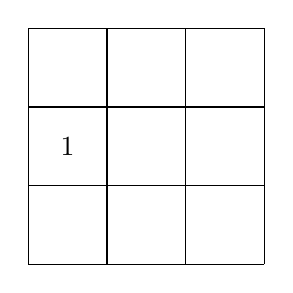
\begin{tikzpicture}
        \draw[xstep=1cm, ystep=1cm] (0, 0) grid (3, 3);
        \node at (0.5, 1.5) {1};
      \end{tikzpicture}
    \end{minipage}
  \fi
  %\ifoutline\outline\par
  %\fi
  %\ifoutcome\outcome\par
  %\fi
\end{exercise}
